In the previous section, we described Ascent's high-level abstractions and
capabilities.
%
This section discusses Ascent's system architecture starting at its inner layer, Flow,
and moving outward.

\subsection{Flow: A data-type agnostic data-flow based architecture}
\label{sec:flow}
Ascent uses a graph-based data-flow architecture.
The data-flow architecture allows Ascent to track, re-use, and cleanup intermediate
results efficiently while implementing complex visualization pipelines.
The design also abstracts how we register and execute operations,
which simplifies adding new features.

At Ascent's core is a simple data-flow library known as Flow, that
composes and executes filters, which are the basic unit of execution in Ascent.
%
Flow is an evolution of a Python data-flow network
~\cite{flow_reference}, but unlike its ancestor, Flow is a C++
library.
%
Flow supports composing and executing directed acyclic graphs
(DAGs) composed of filters~\cite{LarsenAscent}.

There are four components to Flow:
\begin{itemize}
  \item \textbf{Filter}: basic unit of execution.
  \item \textbf{Graph}: contains the filter graph and manages the adding of
filters.
  \item \textbf{Registry}: manages the lifetime of filter results.
  \item \textbf{Workspace}: contains both the registry and filter graph,
coordinates graph execution.
\end{itemize}

\paragraph{Flow Filters}
Flow filters are the basic unit of execution inside of Ascent, and
almost all functionality inside of Ascent is implemented as a Flow filter.
%
Adding new capabilities to Ascent means wrapping that functionality inside
a flow filter.
%
Filters declare an interface, i.e., how many inputs a filter has and
if there is an output, and filters are passed a set of parameters inside
of a Conduit node (see \S\ref{Conduit}).
%
Filter inputs are tracked as arbitrary pointers and runtime features allow
filters to identify and obtain concrete types for processing.
%
In terms of Ascent actions, pipeline filters become part of a chain of
data transformations and would minimally have an input
data set and an output data set, while scenes and extracts
become sinks that have an input data set and no output.
%

\paragraph{Graph}
The graph is a series of Flow filters connected together into
a DAG.
%
The graph is responsible for storing filters and connections
between filters.
%
The primary graph interface supports adding filters and connecting
filter ports (e.g., inputs and outputs) together.

\paragraph{Registry}
The registry is a key-value data store used to manage the intermediate
results of filters inside the data-flow network.
%
Keys within the registry are reference counted, and data contained
inside the registry is deleted when the reference counts reach zero.
%
While the data associated with a key can be a pointer to any type,
the majority of the data stored in the registry are Conduit Nodes
or VTK-m data sets.


\paragraph{Workspace}
The workspace is a container for both the graph and the registry,
and the workspace is responsible for executing the DAG.
%
Additionally, the workspace manages the lists of known filters.
%
A filter must be registered with the workspace in order to be added to the
graph, and once registered, a filter can be added to the graph by name.
%
Flow uses a topological sort to ensure proper filter execution order,
to track all intermediate results, and to provide basic memory management capabilities.
During execution, the workspace provides the registry with reference counts that reflect graph connections, allowing intermediate results to be efficiently managed.

%
Multiple workspaces can co-exist, and in fact, Ascent uses a separate Flow workspace
to evaluate expressions within the Ascent runtime.
%

\subsection{Runtime}
The Ascent runtime builds on top of Flow, and the main responsibility of the
runtime is to translate user actions into data-flow networks.
%
For example, when a user describes a series of data transformations inside of a pipeline,
the runtime adds the corresponding filter for each transformation to
the internal Flow graph.
%
Some actions, like the contour filter, have exactly one filter that the runtime
adds when translating actions, while other actions add more than one filter to the graph.
%
Fig.~\ref{img:flow_graph} shows a simplified view of a data-flow network constructed by the
runtime to create contours of a simulation field and rendering an image of the result.
%

\begin{figure}
\centering
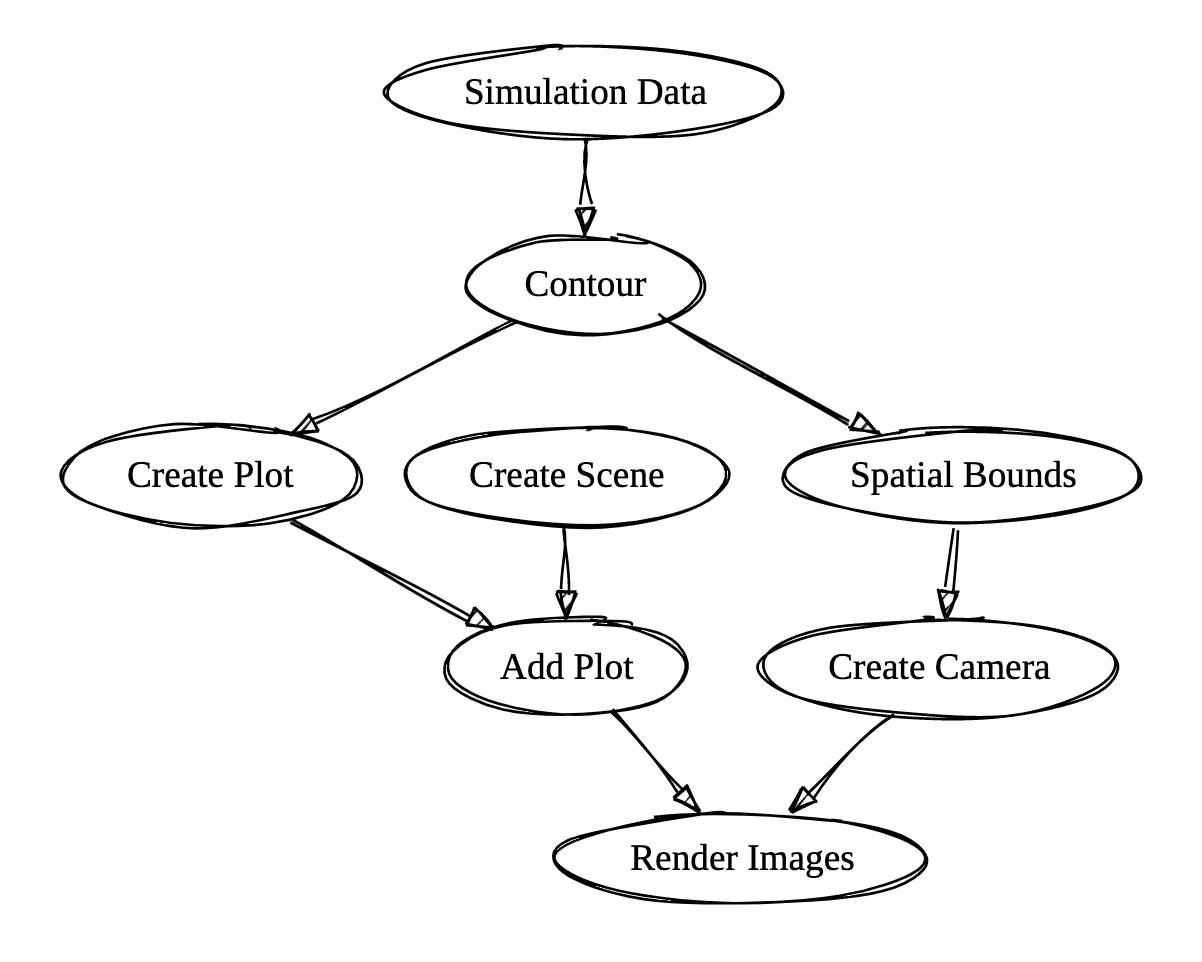
\includegraphics[width=0.6\textwidth]{images/flow_graph}
\caption{\label{img:flow_graph} An example data flow network using Flow assembled by the Ascent runtime.}
\end{figure}

Internally, the runtime maintains a list of registered filters to map
user-facing API names to the corresponding Flow filters which are hidden
from the user.
%
In addition to mapping API calls to Flow filters, the filter map also specifies
in what actions a filter can be used.
%
Runtime Filters can be registered as either a ``transform'' or an ``extract.''
%
Transforms are only callable inside of pipelines and extracts can only be called at the end of a pipeline.
%
Built-in functionality is registered internally with the Ascent runtime when Ascent is initialized.


The runtime also exposes the filter registration of the underlying data flow network which
allows the runtime to inherit Flow's flexibility.
%
Simulations, or other analysis libraries, are free to register custom capability at
runtime, and this allows outside functionality to build off the capability
provided by Ascent.
%
Just like internal filters, custom filters can either be registered as transforms or extracts,
and can directly connect with simulation data or consume the results of a pipeline.
%

The other responsibility of the runtime is to interface with the simulation through Ascent's
main API calls.
%
The runtime consumes configuration options like MPI communicators, exception
handling, and what
backends (e.g., OpenMP or CUDA) to execute code on.
%
Additionally, the simulation's mesh data and the actions are all passed to the runtime.

\subsubsection{Parallelism in Ascent}
Ascent is a hybrid-parallel library, meaning that it uses both
distributed-memory (e.g., MPI) and shared-memory parallelism
(e.g., CUDA and OpenMP), and Ascent is primarily
tightly-coupled with simulations.
%
In the tightly-coupled paradigm, simulations control how parallelism is used, so
it is imperative that Ascent's functionality be capable of running
on the same architectures using the same types of parallelism as the
simulations.
%
Ascent supports many different parallel configurations including
one MPI rank per core (i.e., no shared-memory parallelism), one rank
per GPU, and one rank per node.
%
While Ascent does internally leverage shared-memory parallelism
for expressions, the majority of the shared-memory parallelism comes
from Ascent's components such as VTK-m and Devil Ray.

\paragraph{Distributed-Memory Parallelism}
Within Ascent, all MPI ranks receive the same set of actions.
%
Since the actions are the same, all MPI ranks create and execute the same graph,
meaning that all flow filters execute on all ranks.
%
Ascent guarantees that each filter is given full control of MPI communication,
and filters are free to use MPI anyway they see fit, including
creating asynchronous tasks.
%
Some filters, such as threshold, do not need to use any
MPI communication, i.e., each block of data is processed independently,
but other filters, such as particle advection, use MPI to pass particles
from one rank to another.
%
For mesh data, as discussed in \S\ref{ascent_control},
each MPI rank receives data published by the simulation, and
Ascent does not redistribute the data.
%
That said, filters can change the data distribution (e.g., resampling
an unstructured grid onto a uniform grid), although this can be a costly
operation.
%

\paragraph{Shared-Memory Parallelism}
Ascent's main components use portable performance abstraction layers to
take advantage of the different types of shared-memory parallelism on
modern supercomputers.
%
For example, VTK-m is itself a portable performance layer designed specifically
for visualization and currently supports OpenMP, CUDA, and TBB.
%
Devil Ray, while not itself a portable performance layer, uses RAJA to execute
on different architectures, supporting OpenMP, CUDA, HIP, and TBB.

\subsubsection{Data Set Representations}
Ascent uses an internal data abstraction, called the data object, as the input
and outputs of filters.
%
The data object is responsible for transforming data from one in-memory format
to another without unnecessary copies.
%
By using this abstraction, filters can ask for whatever data set
representation they need, however, the conversions between data
representations are not always one-to-one and may not always
result in a shallow copy.
%

To support multiple data set representations, there must be a common
set of supported features, but not all data models Ascent uses
support the same set of features.
%
Since Ascent uses Blueprint(see \S\ref{Blueprint}) as its data interface to simulations,
all other data models must sometimes be adapted to support additional
features.
%
For example, Blueprint supports multiple topologies in the same data set
but VTK-m only supports a single topology.
%
To handle this correctly within Ascent, we wrap the data sets in a container
that treats each topology as individual VTK-m data sets.
%
